\documentclass[a4paper,12pt,twoside]{article}
\usepackage{graphicx}
\graphicspath{{./images/}}
\usepackage{wrapfig}
\usepackage{pdfpages,caption,geometry} %enables you to add pdf and a caption

\usepackage{geometry}
\geometry{
  a4paper,
  total={170mm,257mm},
  left=20mm,
  top=40mm,
  bottom=30mm,
}

\usepackage{color, colortbl}
\definecolor{Gray}{RGB}{220,220,220}

\usepackage[dvipsnames]{xcolor}
\definecolor{OMDTZblue}{RGB}{0, 166, 225}
\definecolor{OMDTZyellow}{RGB}{253, 214, 14}
\definecolor{OMDTZgreen}{RGB}{19, 186, 42}

\usepackage{sectsty}
\sectionfont{\color{OMDTZblue}} 
\subsectionfont{\color{OMDTZblue}}
\subsubsectionfont{\color{OMDTZblue}}

\usepackage{caption}
\usepackage[font={color=OMDTZgreen,small,bf},figurename=Fig.,labelfont={small,it}]{caption}
\usepackage{subcaption} 

\usepackage[utf8]{inputenc}
\usepackage[english]{babel}
\usepackage{multirow}
\usepackage{multicol} % Allows multiple columns to be used on the fly

\usepackage{fancyhdr}
\pagestyle{fancy}
\fancyhf{}
\lhead{\color{black} \leftmark}
\rhead{\color{black} \rightmark}
\fancyfoot[LE]{\color{black} \thepage \hspace{5mm} \scriptsize Innovation Ecosystem Map---1st Quarter Report}
\fancyfoot[RO]{\color{black} \scriptsize Innovation Ecosystem Map---1st Quarter Report \hspace{3mm} \normalsize \thepage}

\newcommand*{\vcenteredhbox}[1]{\begingroup
\setbox0=\hbox{#1}\parbox{\wd0}{\box0}\endgroup} % For creating vertically centered rows of logos

\setcounter{tocdepth}{2} % Table of Contents includes only sections and subsections, not subsubsections.

\usepackage[framemethod=tikz]{mdframed}% adding a shadow to a text for emphasis
\usepackage{lipsum}

\usepackage{hyperref}
\hypersetup{
  colorlinks=true,
  linkcolor=OMDTZblue, % to match the OMDTZblue text
  filecolor=magenta,      
  urlcolor=cyan,
  pdftitle={Innovation Ecosystem Map---1st Quarter Report},
  bookmarks=true,
  %pdfpagemode=FullScreen,
}
%\urlstyle{same}


\usepackage[english,ngerman]{babel}
\usepackage[T1]{fontenc}% font package

\usepackage[scale=1]{helvet} % or tgheros
\renewcommand{\familydefault}{\sfdefault}

\usepackage{bbding}% used for adding symbols e.g. checkmark


\begin{document}

\thispagestyle{empty}

\begin{center}
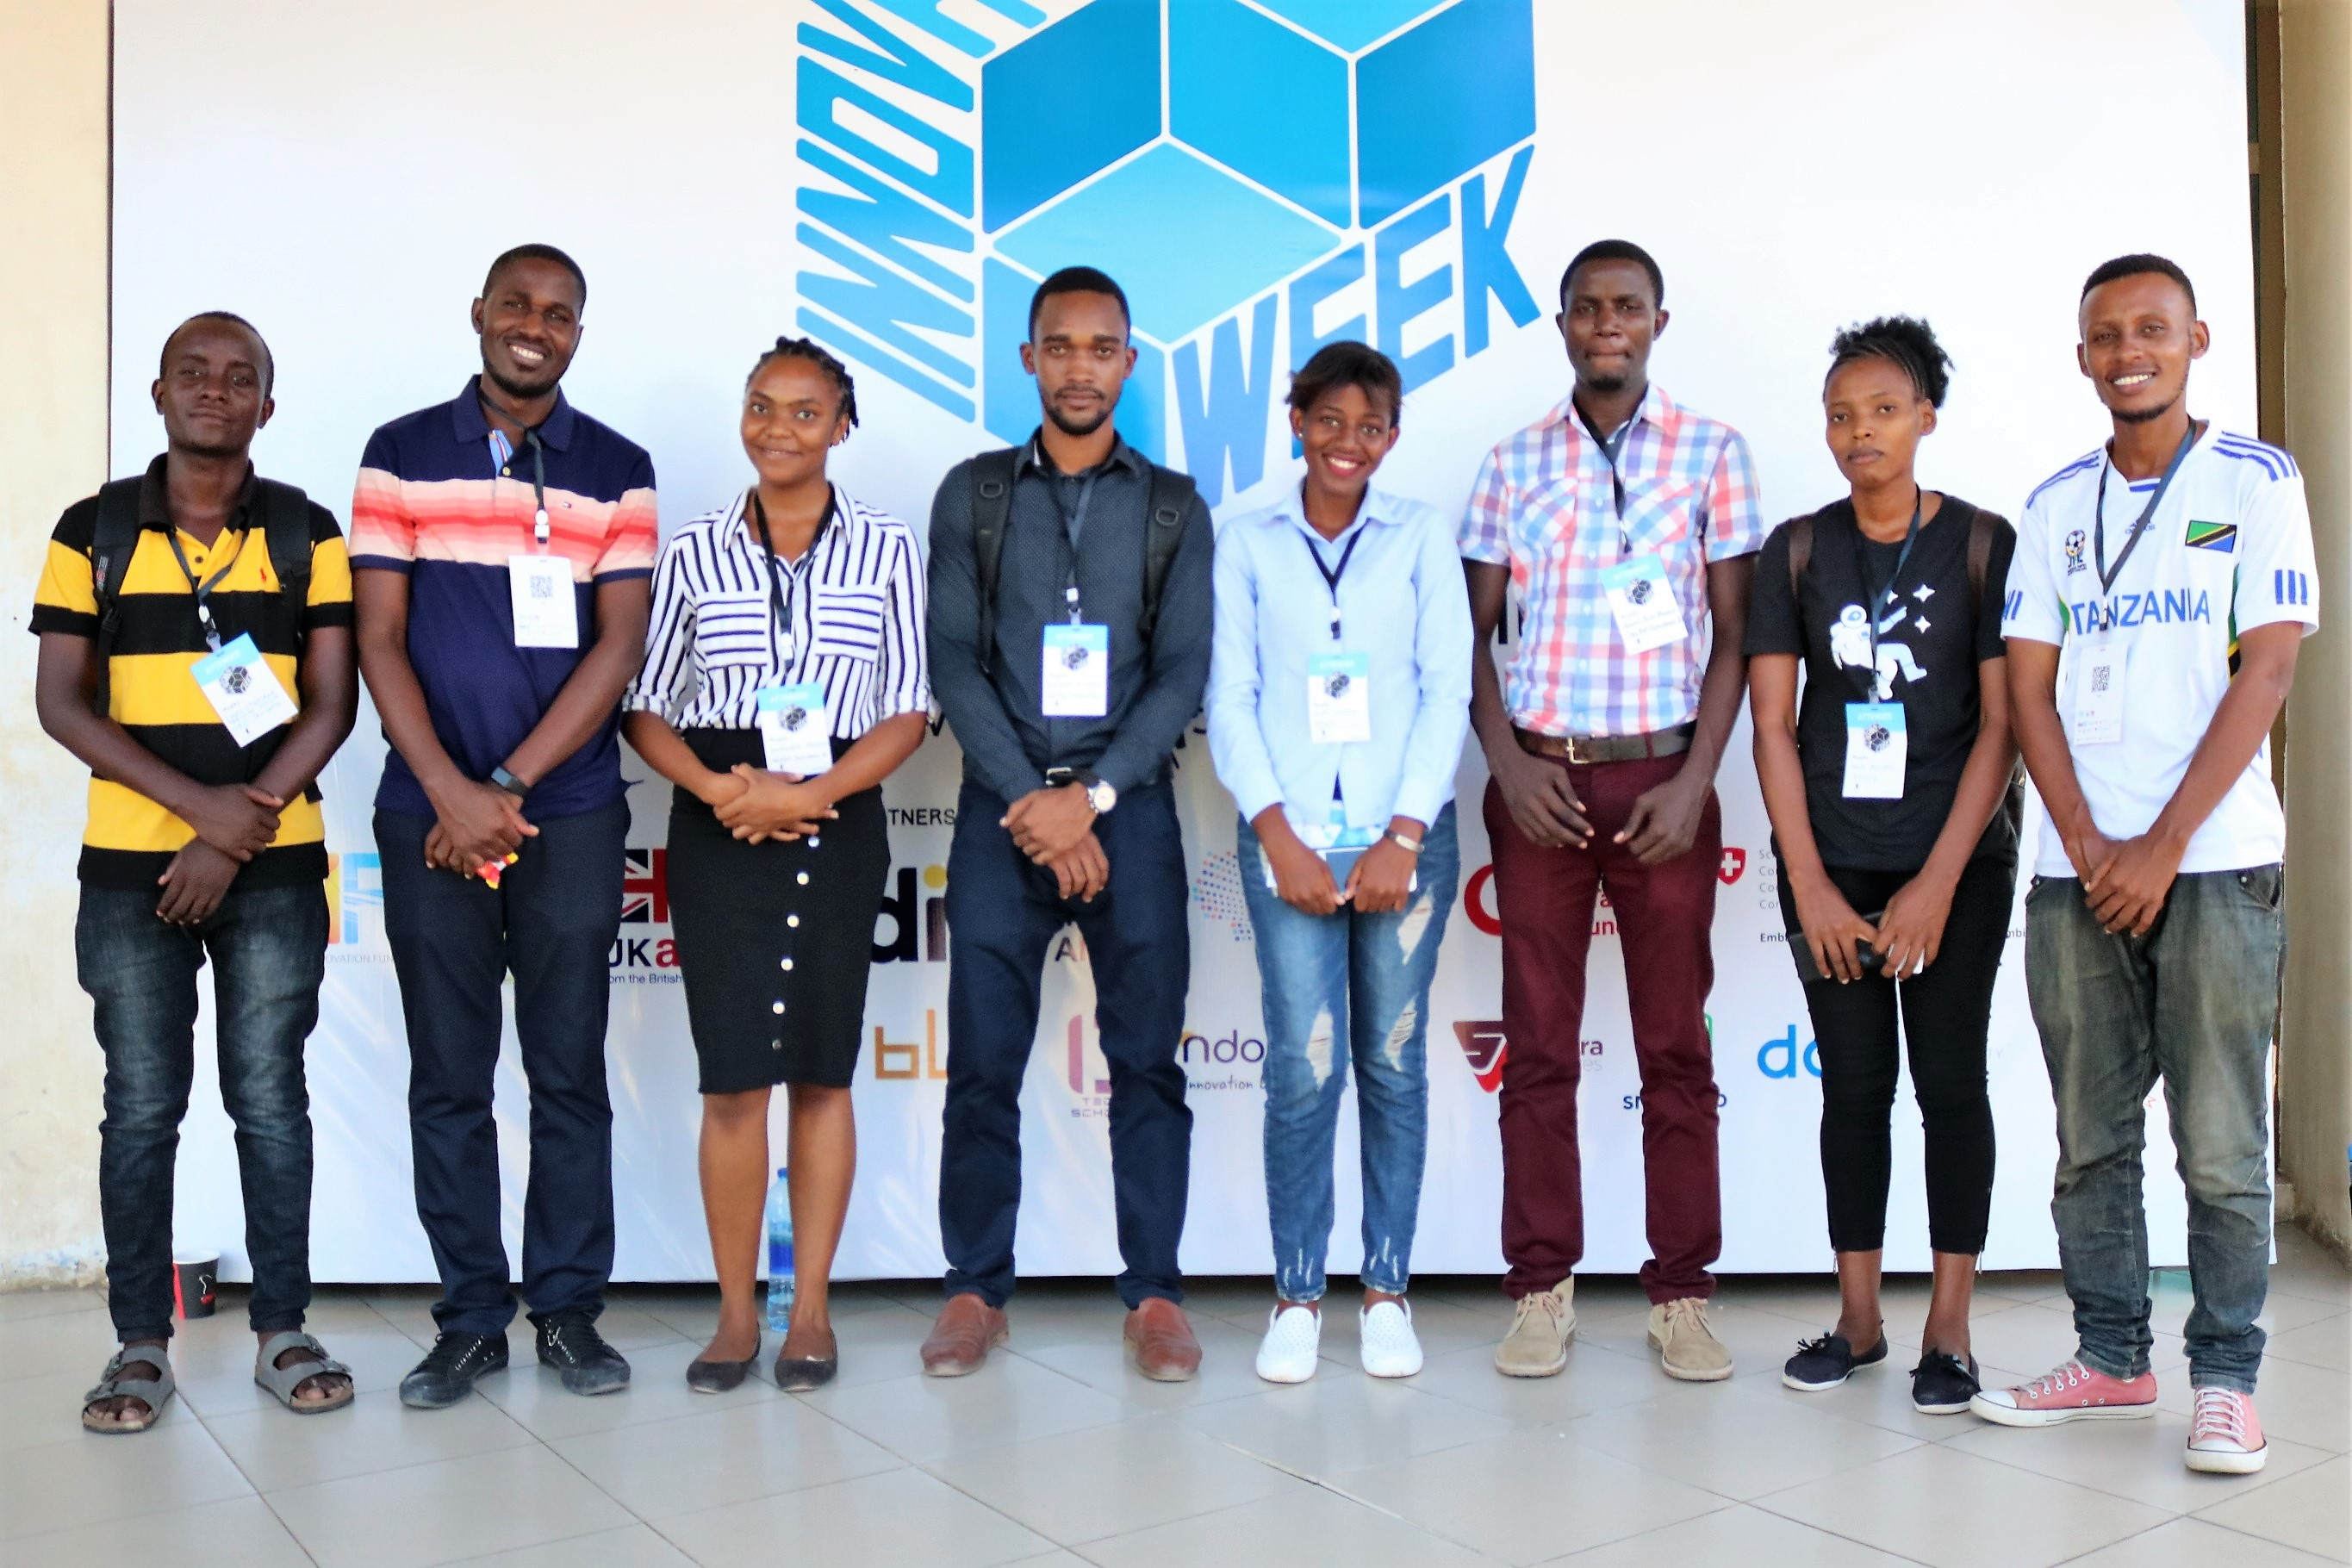
\includegraphics[width=\textwidth]{Group_shot.JPG}
\end{center}

\begin{center}
\bigskip
  \Huge 
\color{OMDTZblue} \textbf {Innovation Ecosystem Map}
\\
\textbf{Project Progress Report}
\\
\end{center}
\bigskip \bigskip \bigskip
\\
  \vbox{
  \centering
  Prepared for:
  \vcenteredhbox{
\includegraphics[width=2cm]{images/hdif_logo_new.png}}
  \
  by:
  \vcenteredhbox{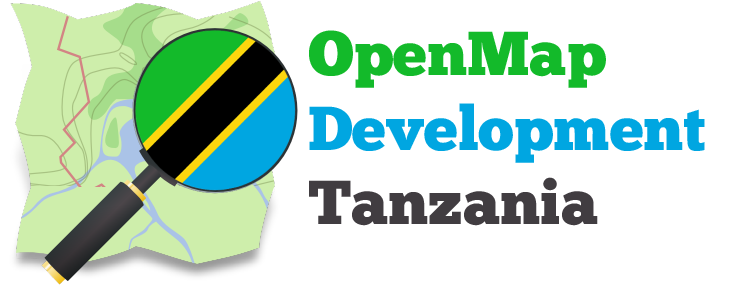
\includegraphics[width=4cm]{images/OpenMap_Development_TZ_Logo_Security_Card.png}}
  % \maketitle
}
\bigskip  \bigskip \bigskip
\begin{center}
  March 2019, Dar es Salaam, Tanzania  
  
 \bigskip \bigskip \bigskip \bigskip \bigskip \bigskip
 
\footnotesize {Authors: Wombura Kimacha, Johanes Peter, Hawa Adinani, Immaculate Mwanja and Innocent Maholi}
  
\end{center}

\newpage
\tableofcontents
\newpage
\section{Summary}
This report describes the first quarter of the Innovation Ecosystem Map of Tanzania Project supported by the \href{http://www.hdif-tz.org/}{Human Development Innovation Fund (HDIF)}\footnote{\url{http://www.hdif-tz.org/}} and led by \href{http://omdtz.or.tz/}{OpenMap Development Tanzania (OMDTZ)}\footnote{\url{http://omdtz.or.tz/}}.
\bigskip

It provides an in-depth description of the activities done from January to March of 2019, what we have learned so far from the engagement with stakeholders and an evaluation of the sustainability models of the Innovation Ecosystem Map of Tanzania. 
\bigskip

To begin the project, OMDTZ sat down with HDIF several times to understand the background and objectives of the project. This was followed by two trainings of trainers (TOTs), so that the OMDTZ team could become familiar with the innovation categories. In addition, we discussed the complexity around defining “innovation” as well as the strategic value of the map.
\bigskip

Informed by these discussions, OMDTZ created a data model in order to structure all of the key information necessary for building the map. This was then used to design a mobile survey form that will assist in the data collection phase.
\bigskip

During Innovation Week, we gave a workshop to introduce the map as well as OMDTZ to provide visibility and awareness of both. This was followed a few days later by a Hub Managers Workshop, that was successful at generating conversation around the challenges within the ecosystem and ideas about how to overcome them.
\bigskip

By the end of this quarter, OMDTZ faced several challenges and learned important lessons that will guide the project moving forward. For instance, through discussions with stakeholders, it was documented that some of the innovation categories were missing, which reflects a gap within the current model that will allow us to capture additional innovators. As a lesson, this has to be given a good thought in acting as too many categories will make the map fragmented with many options which will make the map more difficult to use.
\bigskip

On a general note, the first quarter has been incredibly useful for OMDTZ to understand the ecosystem and begin making connections within it. It is clear that we will need to work closely with stakeholders so they understand the value of the map and realize its potential to improve connections and collaboration between them and investors. 



\newpage
\section{Project Narrative}
\subsection{Background}
HDIF initiated a process in 2016 to run a study of the Tanzanian innovation ecosystem and to document the ecosystem players on an online map platform, accessed \href{http://innovate.co.tz}{here}\footnote{\url{http://innovate.co.tz}}. The goal of the mapping was to increase HDIF and innovation stakeholders’ understanding of the key players and actors in the innovation ecosystem, with the aim of improving connections and collaboration between players to help inform future programming, and to understand the landscape and gaps in the innovation sector.
\medskip

The first phase of the map was managed by ANZA---an innovation organisation, founded on the belief that entrepreneurs will transform Tanzania. Through this time, ANZA was able to map and enlist more than 400 stakeholders of the innovation ecosystem in the country. As shown from the data collected, a huge share of the ecosystem is dominated by the coastal zone of Tanzania which dominates 41.1\% of the ecosystem and the least is the Western zone which dominates only 3.5\% of the distribution. A need to increase the number of stakeholders is vital to ensure as many stakeholders as possible exist on the map and to facilitate easier interaction among them.
\medskip

It wasn’t until 2019 that the project transformed into its second phase, awarded to OMDTZ---a successor that has been tasked to:
{\renewcommand{\theenumi}{\roman{enumi}}%use package for roman numbers
\begin{enumerate}
    \item Administer the map through creating awareness and populate the map.
    \item Create community ownership through mapping parties, workshops and webinars.
    \item Review and improve the map technology. 
\end{enumerate}}

\subsection{Primary Objective}
We are focusing on administering and managing the innovation map as a platform to bridge the gap and provide a conducive environment and linkages among innovation stakeholders in the country. The end goal is to build the map into a sustainable platform to support the Innovation Ecosystem of Tanzania.

\newpage
\section{Milestones}
This section provides an overview of the project status with regards to conducted activities and their progress as well as describing the milestones.

\subsection{Creation of a Data Model}
This is an abstract model that organizes elements of data and standardizes how they relate to one another and to properties of real-world entities. The development of a new data model was required in order to make sure all necessary information about stakeholders in the ecosystem are collected. The process of creating a new data model involved different stakeholders with the aim understanding the necessary information on the map as well as initiate discussions on the innovation categories. This was initially done through visits to HUB255, Sahara Ventures, Hype Interactive etc., and the discussion was later expanded during the Innovation Week 2019 when OMDTZ engaged with Hub managers and the stakeholders to discuss the categories in depth. The discussions eventually led to the development of the data model that is currently being used. The role of the data model is to inform and guide questions to be asked when collecting data via \href{innovate.co.tz}{innovate.co.tz} and OpenDataKit Collect.

Key information included in the data model are the location, address and contact information, social media, parameters information and other additional information. 

A created data model can be accessed \href{https://docs.google.com/document/d/1aF2kEEGu6Kf91UlXY6L8WYJblrPpesggKiJCtD9nvZ4/edit?usp=sharing}{here}\footnote{\url{https://docs.google.com/document/d/1aF2kEEGu6Kf91UlXY6L8WYJblrPpesggKiJCtD9nvZ4/edit?usp=sharing}}: A summary of the data model is shown below:

\newpage
\begin{center}
    \large Summary of the Data Model
\end{center}
\begin{multicols}{3}
\begin{mdframed}[hidealllines=true,backgroundcolor=OMDTZgreen!10,innerleftmargin=6pt,innerrightmargin=6pt,leftmargin=-3pt,rightmargin=-3pt]

\textbf {Survey Information}
\begin{itemize}
    \item start
    \item end
    \item today
    \item username
\end{itemize}
\textbf {Location Information}
\begin{itemize}
    \item region
    \item district
    \item ward
    \item street
    \item landmark
    \item geopoint
\end{itemize}
\end{mdframed}
\begin{mdframed}[hidealllines=true,backgroundcolor=OMDTZgreen!10,innerleftmargin=6pt,innerrightmargin=6pt,leftmargin=-3pt,rightmargin=-3pt]
\textbf {Address and Contact}
\begin{itemize}
    \item name
    \item postal address
    \item telephone number
    \item fax number
    \item email address
    \item website
\end{itemize}
\textbf {Social Media Information}
\begin{itemize}
    \item LinkedIn
    \item Twitter
    \item Facebook
    \item YouTube
    \item Instagram
    \vfill\null
    \columnbreak
\end{itemize}
\end{mdframed}
\begin{mdframed}[hidealllines=true,backgroundcolor=OMDTZgreen!10,innerleftmargin=6pt,innerrightmargin=6pt,leftmargin=-3pt,rightmargin=-3pt]
\textbf {Parameters Information}
\begin{itemize}
    \item categories 
    \item sectors served
    \item target groups
    \item services offered
    \item mode of payment
\end{itemize}
\textbf {Additional Information}
\begin{itemize}
    \item description
    \item certificate
    \item logo
    \vfill\null
\end{itemize}
\end{mdframed}
\end{multicols}


\subsection{OpenDataKit Form}
This is a form standard created to help simplify the authoring of survey forms in Excel (.xlsform). The form replaces usage of papers and makes the whole process of data collection eco-friendly and simplifies analysis. The form was created by reflecting the data model created by OMDTZ. Questions in the survey form flow in a manner that captures all required information about a company or organization.
\medskip

ODK Collect supports different file formats such as location, audio, images, video, barcode scanning, signatures, free texts, multiple choice, and numeric answers. The application was used to test the developed ODK survey that will be used for field data collection in the second quarter.
\medskip

The form includes a total of 30 questions, with skip-logic conditions that depend on the selection of the previous questions. One of the lessons learned from the first stage of the map is self-identification of the innovators which raised several issues including individuals mapping themselves even though not belonging to any of the innovation categories etc. With the current map and the use of ODK collect for data collection, the issues are currently being addressed and solutions to the problem are developed right before we conduct data collection.
\medskip

Having said so, above are two screenshots of ODK Collect interface displaying the questions.
\begin{figure}
\centering
  \begin{subfigure}[b]{0.3\textwidth}
    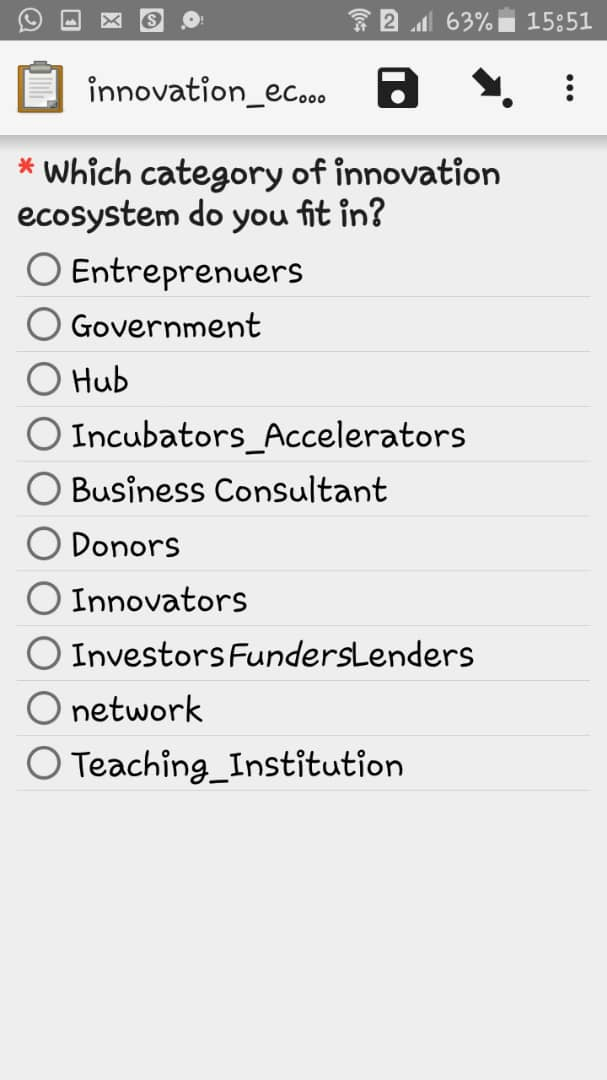
\includegraphics[width=\textwidth]{images/ODK_1.jpeg}
     \color{OMDTZgreen}\caption{ODK Collect form choices category}
    \label{fig:1}
  \end{subfigure} \hspace{10mm} %\hfill or \hspace{0.3\textwidth}
  \begin{subfigure}[b]{0.3\textwidth}
    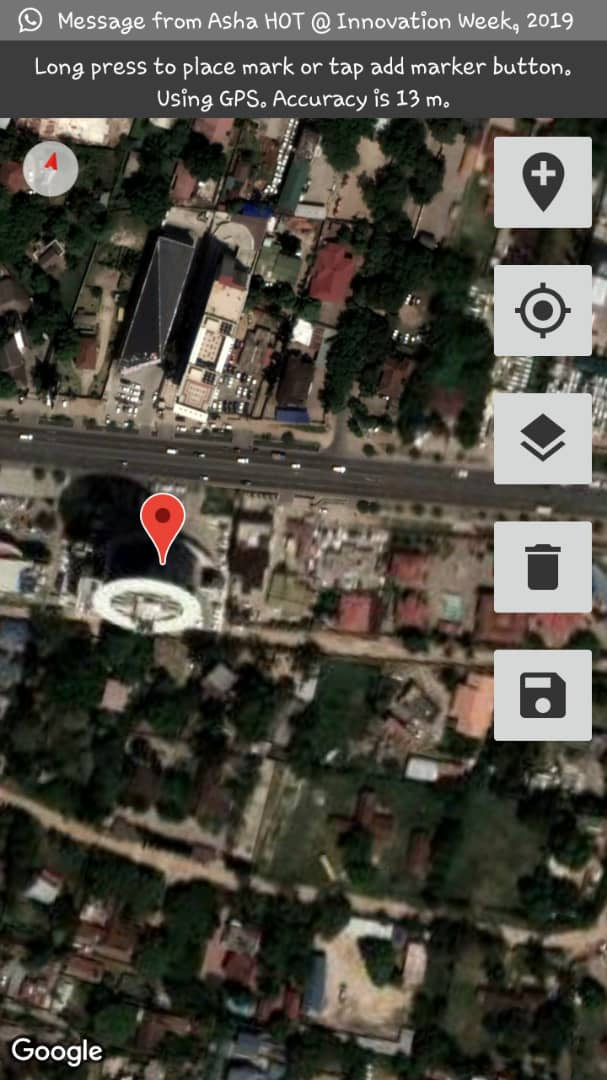
\includegraphics[width=\textwidth]{images/ODK_2.jpeg}
    \color{OMDTZgreen}\caption{Aerial imagery as dispayed in ODK Collect}
    \label{fig:2}
  \end{subfigure}
\end{figure}

\subsection{Training of Trainers}
OMDTZ, in collaboration with HDIF, conducted training for both the trainers and trainees which took place on 25th and 29th of January 2019. The training was collaborative as it provided the room for interaction for every participant to make comments and suggestions on the categories and redefine them on the map.
\medskip

The first training took place at HDIF’s offices with Kristiina Lahde leading the training and supported by Alexa du Plessis and  Simon Mutabazi.
\medskip

The focus of the training was based on:

\begin{itemize}
    \item Defining the strategic value for the Map---why it is viable, what are the impacts and potential benefits to stakeholders in the ecosystem.
    \item Share the mapping methodology
    \begin{itemize}
        \item Making sure we have a similar understanding of the current map categories; reformulating the definitions jointly if needed, modifying the categories if needed.
        \item Discussing the information collection plans in detail, whether OMDTZ needs help in planning the training for data collectors etc.
    \end{itemize}
    \item An overview of the Principles for Digital Development
    \item Planning the innovation week events
\end{itemize}

\begin{figure}[h]
  \caption{Training of Trainers at HDIF}
  \centering
  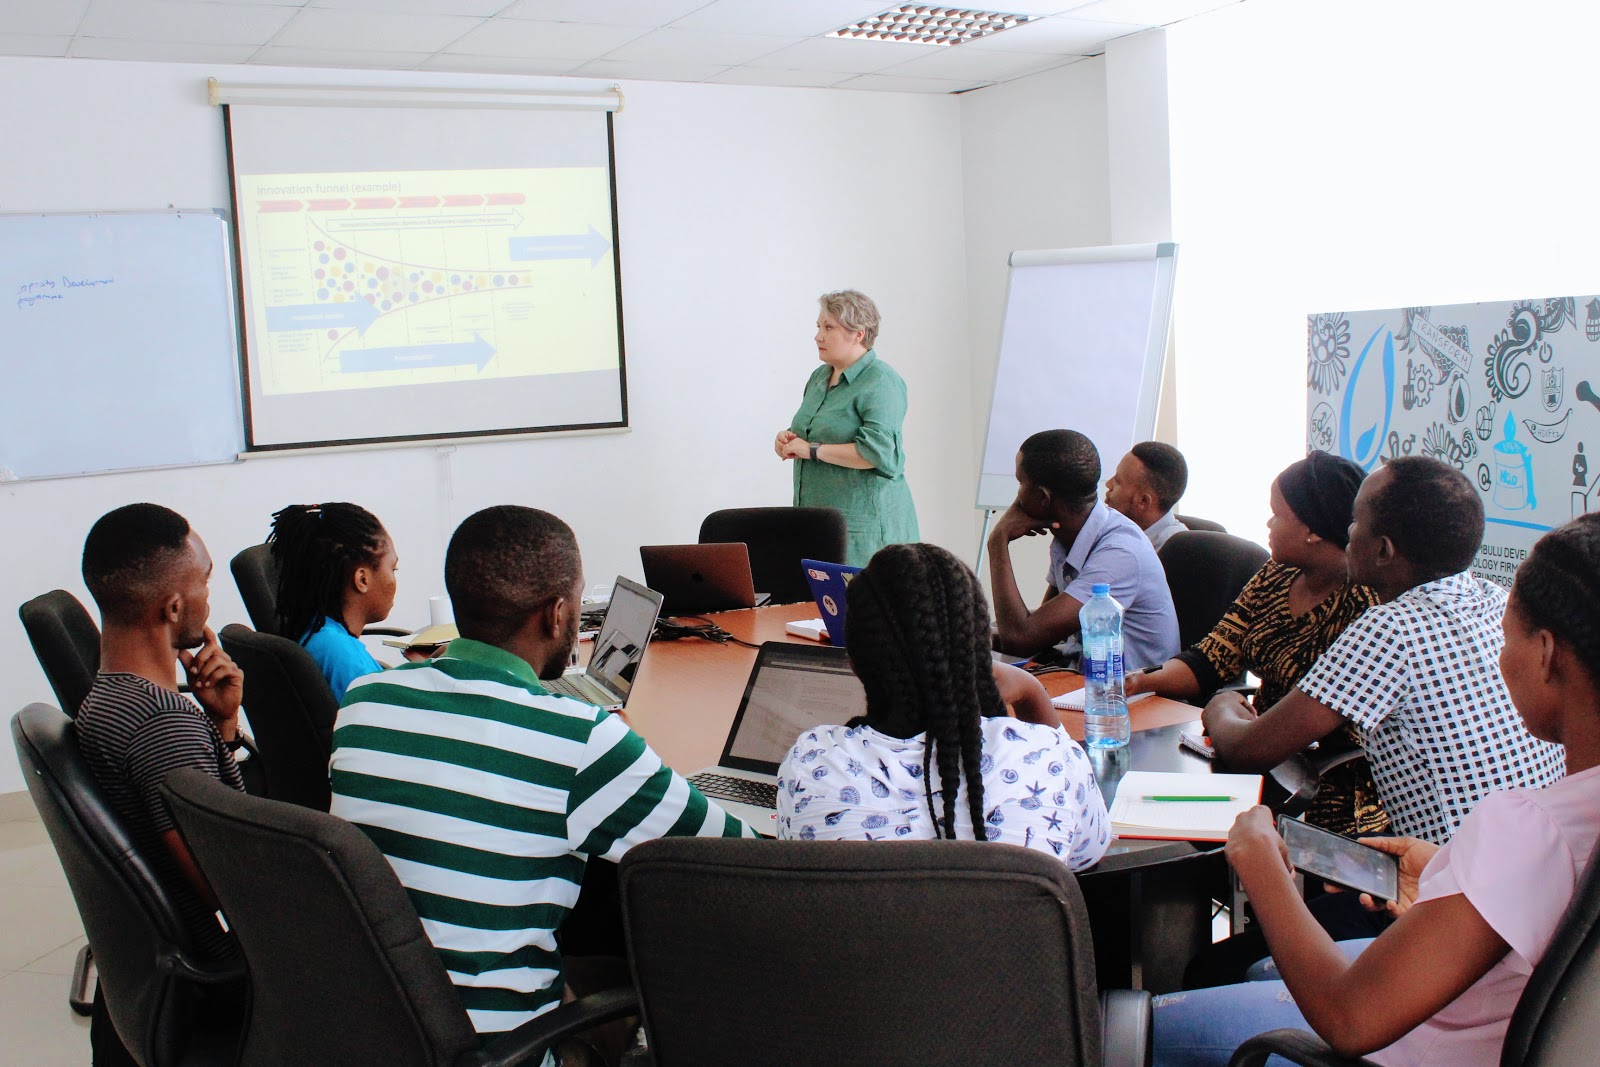
\includegraphics[width=0.6\textwidth]{images/HDIF_training.jpg}
\end{figure}

The second training took place at OMDTZ’s office and it was attended by 8 participants working with OMDTZ. The training was meant to make a review of the previous training at HDIF and make sure that the trainers are on the same page on the categories and strategic values of the map.
\medskip

Trainees were given sticky notes and asked to give their views/ideas on how they think the stakeholders are going to use the map.

\begin{figure}[h]
  \caption{The sticky notes were grouped into 8 categories and clustered into groups}
  \centering
  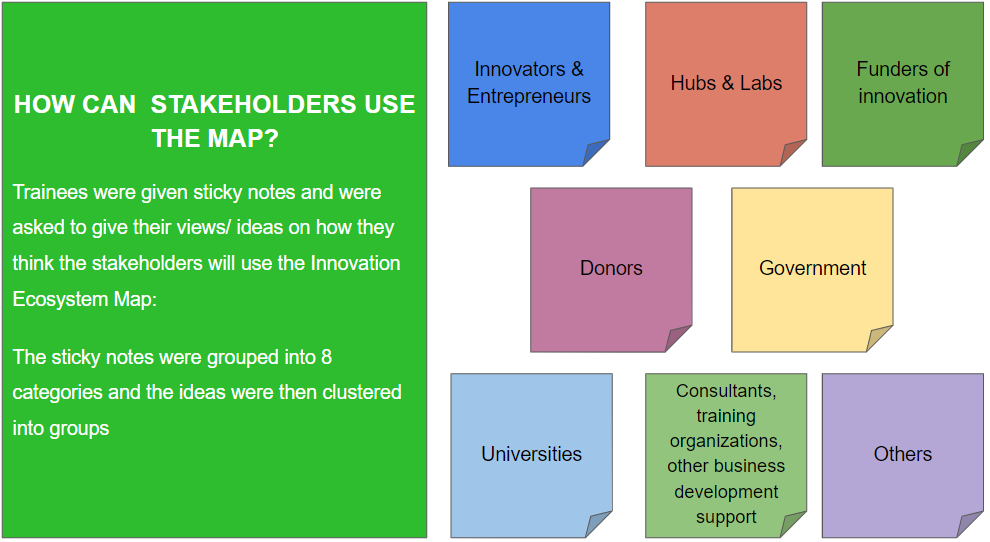
\includegraphics[width=0.6\textwidth]{Strategic_value_PPT.PNG}
\end{figure}

The strategic values of the Map can be found \href{https://docs.google.com/presentation/d/1rm31zWGpLR9yI7V2yYEwL8GoHprIDP_VGHo9Zufjkn8/edit#slide=id.g4e94bd219a_0_2}{here}\footnote{\url{https://docs.google.com/presentation/d/1rm31zWGpLR9yI7V2yYEwL8GoHprIDP_VGHo9Zufjkn8/edit#slide=id.g4e94bd219a_0_2}}

\subsection{Innovation Week 2019}
This was a week-long series of events hosted by Human Development Innovation Fund (HDIF) and COSTECH with support from UKAid. This year’s innovation week took place from the 25th - 30th of March with a theme “Scaling and Sustaining Innovation for Human Development”. OMDTZ participated by showcasing and having interactive discussions on the “Innovation Ecosystem Map of Tanzania” through workshops and exhibition. 

\subsubsection{Workshop on 25th March}
The first workshop was held on the 25th of March at Rotunda Hall - COSTECH, and was attended by 32 participants from various innovation backgrounds. This was a two-hour session with the contents; 

\begin{itemize}
    \item Introduction and history of the map by HDIF’s Strategic Partnership Advisor - Alexa Du Plessis.
    \item OMDTZ’s tasks on innovation ecosystem map.
    \item Potential application of the map, an interactive session with participants.
    \item Mapping training with ODK collect.
    \item Discussions with Q&As.
\end{itemize}

The session bore good feedback on refining the criteria for categories, better ways to connect with the stakeholders, and the importance of reviewing the map technology especially on filtering information.

\subsubsection{Workshop on 27th March}
The second event was termed as a “Hub Managers Workshop” held on the 27th of March at Seedspace and was attended by 25 managers from different hubs across Tanzania. This had the following content;

\begin{itemize}
    \item Introduction to the map
    \item Workshop; why is HDIF supporting it and why hubs should care.
    \item Categories presentation and discussions with Q&As.
    \item Next step plan for hubs
\end{itemize}

What we learned is that a number of hub managers were already familiar with the map  even though not clearly, while for a few of them it was their first time to hear about the map. The feedback received from hub managers was very constructive, including the need to re-review the innovation categories as well as OMDTZ should expect cooperation from the hubs on how to improve the map. One of the hub manager offered development support for the new platform which we will discuss later under the Sustainability section. 

\begin{figure}[h]
  \centering
  \caption{Hub Managers Workshop}
 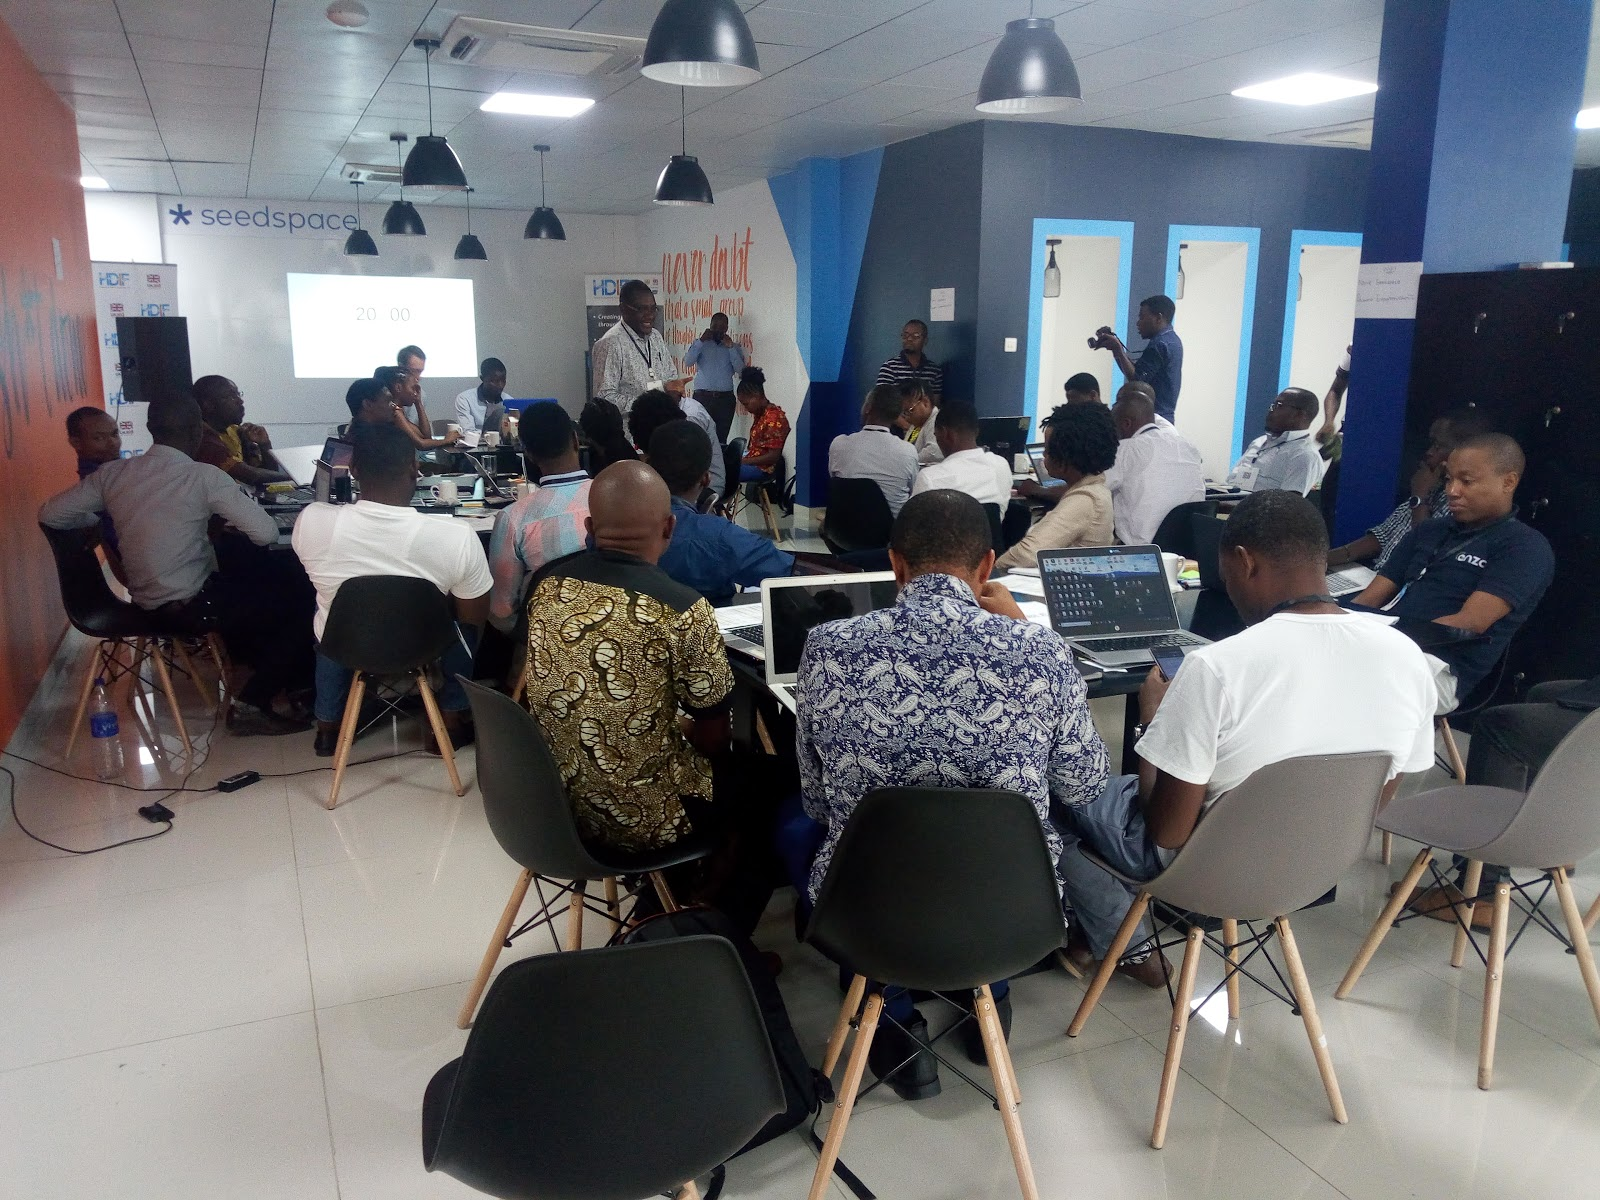
\includegraphics[width=0.6\textwidth]{images/seed_star_workshop.jpg}
\end{figure}

\subsubsection{Exhibition on 29th March}
On the last day of the Innovation Week 2019, OMDTZ held an exhibition of the map. General audience had the chance to learn about the map and experience it at the showcasing booth. Many appeared to be interested with the idea and wanted to know the ways they could be part of the map. \textbf{Our general takeaway on attending the IW2019 was the fact that the map was not known to many of the general audience, the reaction was that innovation stakeholders in Tanzania truly need it.}

\begin{figure}[h]
  \centering
  \caption{Innovation Week Exhibition}
  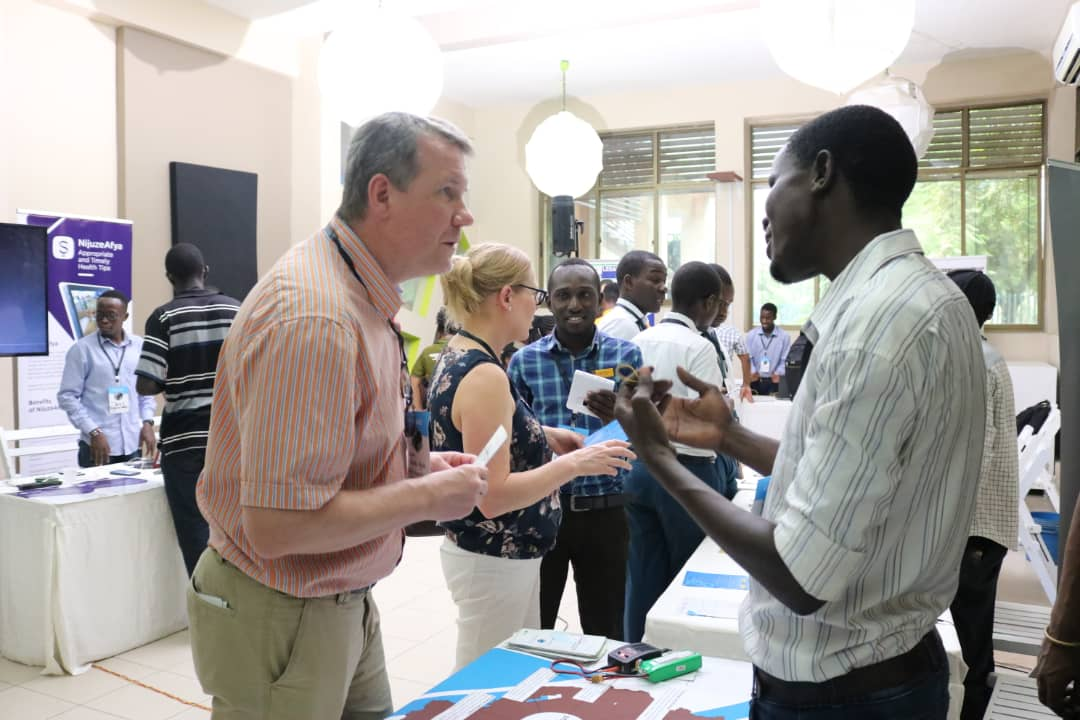
\includegraphics[width=0.6\textwidth]{images/seed_star_training.jpeg}
\end{figure}

\newpage
\section{Challenges and Lessons Learned}
\begin{itemize}
    \item \textbf{Sustainability of using ODK as a data collection tool:}
\end{itemize}
From a series of discussions that we have had with hub managers and other stakeholders, the usage of ODK Collect \textit{(an android data collection app)} as a data collection tool to populate the map will increasingly lead to complexity of data collection and management. Compared to using the online map editing tool, the use of ODK Collect seems to pose extra complexity in dealing with data collection in the fields and managing the servers that are to be linked to the map. The idea here is to use a very easy and user-friendly tool, and together with the hub managers, we all agreed that we should try to collect data through using the online innovation map editing tool which is expected and designed to be user-friendly. user-friendly.

\begin{itemize}
    \item \textbf{Missing innovation categories:}
\end{itemize}
From the engagement with hub managers, we came to learn that a lot of categories to describe the innovation stakeholders were missing. For example, a hub manager from Any Change Lab suggested adding this hub sub-category to our data model i.e. \textbf{Change labs}---these are labs formed for a specific system change, work with local village people to find out what is perishing from the community and to decide what they want to be added to the community. They are also referred to as Social Innovation Labs. As OMDTZ, our wayforward is to wisely try to discuss these issues with HDIF and see if we can fit the new introduced categories into what is existing already. We will also try to follow-up back with the hub managers on the categories etc.

\begin{itemize}
    \item \textbf{The need for verification of Stakeholders:}
\end{itemize}
Verifying innovators and entrepreneurs entries is one of the most important step of the process. Without valid data on the platform, it is quite easy to lose trust from users. An entrepreneur with bad intentions for example might register his/her fake company with the aim of conning other users on the platform. Therefore, this will be dealt as follows;
    \begin{itemize}
        \begin{itemize}
            \item Innovators will be asked to upload a copy of certificate of registration and registration numbers to verify that their organizations are locally or internationally registered.
            \item Before rendering the innovators on the map, there will be a validation process that involves calling/emailing the innovators for further confirmation.
        \end{itemize}
    \end{itemize}

\newpage
\section{Sustainability}
This section describes measures that will be taken into account to ensure that the Innovation Ecosystem Map of Tanzania can sustain itself throughout its lifetime. These include how  the engagement of stakeholders with the map will be maintained, forming partnerships with several stakeholders who are ready to offer support in several aspects for the map and ways that the map can generate funds for its management. From the list below, while some of the measures were inherited from the “RFP for the \href{innovate.co.tz}{innovate.co.tz} map tender”, most of the rest were brainstormed by the OMDTZ team with reference to the experience the team has had with other projects. These are as follows;

\subsection{Platform}
\begin{enumerate}
    \item Creating social media presence for the map and marketing it online. OMDTZ will create Twitter and Facebook accounts with a YouTube channel for sharing the tutorials. While  these will be managed by OMDTZ, they will be branded as the map’s properties (see an example of \href{https://twitter.com/innovationmaptz}{innovation ecosystem map on twitter}\footnote{\url{https://twitter.com/innovationmaptz}}---this has not been promoted as of now).
    
    \
    A dedicated medium blog for the map will be created on the medium platform and will be updated regularly with innovation ecosystem news and events, short interviews etc. The medium blog will also be linked to the map.

    \item A number of stakeholders who show great interest towards the map and are ready to support the map activities will be championed to ensure that the stakeholders take ownership. These are preferably the hubs that can provide an environment---including physical spaces to create awareness of the map and ensure a stronger presence in the ecosystem through organizing mapping event. OMDTZ will work closely with the champions to ensure succession of the map.
    \item OMDTZ will offer a range of mapping party events/workshops with the aim of connecting stakeholders who provide funds, resources and the innovators who implement the projects. These events will help to increase awareness of the map in the ecosystem. Currently, the plan is to work with the hubs to jointly organize these events with OMDTZ.
    \item OMDTZ will host webinars with the aim of training and educating stakeholders on how stakeholders can map themselves and offer an opportunity for the stakeholders to get involved with the map. Webinars will provide a chance for stakeholders to learn about the state of the map, growth of innovation in several sectors and distribution of innovative products among sectors.
    \item OMDTZ will create tutorials on how stakeholders can put themselves on the map. These will be uploaded and shared through the YouTube channel dedicated for the map.
\end{enumerate}

\subsection{Financial Models}
To ensure a constant generation of income to manage the map, ideas proposed are as follows:
\begin{enumerate}
    \item The map will offer a feature to display ads for  stakeholders of the ecosystem and people that want to market themselves on the website. The ads will primarily show the information of advertisers which will be visible to all users of the website. To reduce too much ads traffic, management control will be put by OMDTZ as publishers in place so that these don’t take over the meaning of the website. 
    \item The map will offer featured entries, this is a paid option that will ensure an entry stands out from the rest of the features once a user searches for a particular category. In addition to that, there will be a way for the entries to get featured on the homepage, social media channels, or in the next newsletter.
    \item The blog will dedicate a page for promoting programs and events that aim at bringing together stakeholders of the ecosystem. This will provide a way to reach out to the innovation community and get the best ones to apply for the programs, competitions or funds run by donors/funders.
\end{enumerate}

\subsection{Strategic Partnership Models}
These are the agreements between two organizations where one organization offers support to the counterpart. In managing the map, a partnership with COSTECH---a parastatal organization which maintains a system of collaboration, consultation and cooperation with parties within Tanzania whose functions relate to the development and application of science and technology---will be established.
\medskip

The broader purpose of the MOU will be to enable OMDTZ and COSTECH to develop and expand a framework of cooperation to help in structuring the working relationship between the two parties and to further the aim of supporting innovation community in Tanzania.

\
To mention a few, partnership with COSTECH will fulfill the following goals;
\begin{enumerate}
    \item We believe that COSTECH---the expected biggest user of the map with a mission to foster knowledge-based-economy through promotion, coordination of research, technology development and innovation for sustainable development in Tanzania---will therefore provide support to OMDTZ in acquiring;
    \begin{enumerate}
        \begin{enumerate}
            \item Mapping permits for data collection.
            \item Access to the existing database by COSTECH to add and validate more information collected from the fields.
            \item Endorsement to the use of map by the stakeholders in the innovation ecosystem.
        \end{enumerate}
    \end{enumerate}
    \item In turn, OMDTZ will be able to populate and update the map and the database by COSTECH, which will provide COSTECH with up to date information about the innovation stakeholders etc.
\end{enumerate}
This is still work in progress, and the goals of the MoU are expected to deep dive into enabling good fostering environment for the innovation ecosystem map.

\subsection{Financial Reporting}
The financial report for this project can be seen in the break-down below:

\begin{figure}[h]
  \centering
  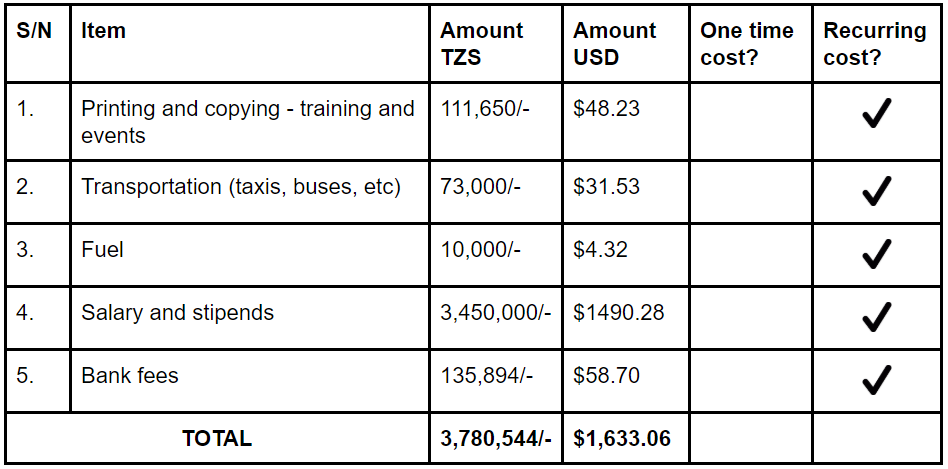
\includegraphics[width=0.95\textwidth]{Financial_model2.PNG}
\end{figure}

\begin{center}
\begin{tabular}{|c|c|c|}
\hline
 & TZS & USD \\
 \hline
 \rowcolor{Gray}
Opening balance & 0 & \$0.00 \\

Amount advanced & 7,402,000/- & \$3,197.41 \\

\rowcolor{Gray}
Amount spent & 3,780,544/- & \$1,633.06 \\

Balance in bank account + cash on hand & 3,621,456/- & \$1,564.34 \\
 \hline
\end{tabular}
\end{center}


\end{document}


%\begin{figure}
%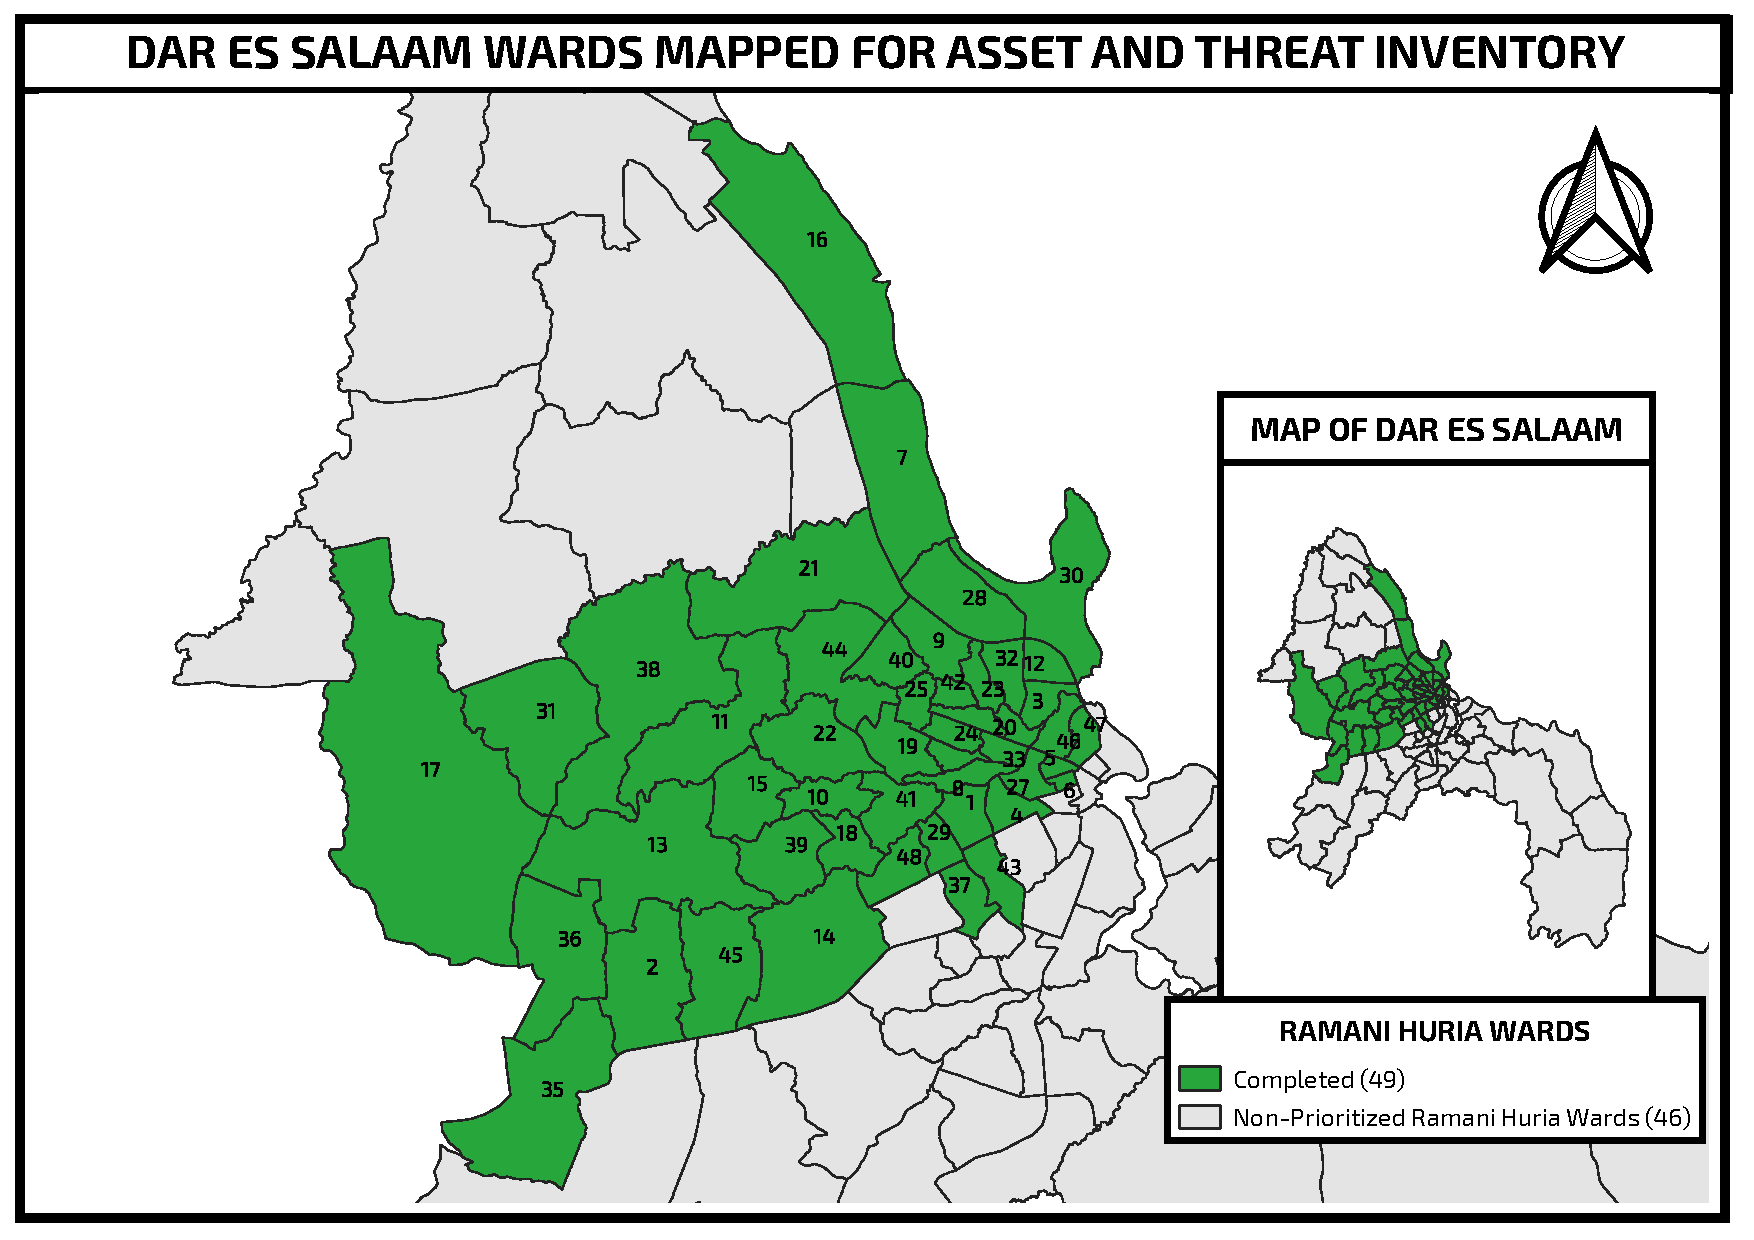
\includegraphics[width=\columnwidth]{images/Asset&Threat.pdf}
%\caption{Image A}
%\end{figure} for adding .pdf files